% Provenance (never printed): see sources/outline_sources.md (Year 3: the main
% field and its secular variation, rock magnetism, palaeomagnetic poles, apparent
% polar wander, magnetostratigraphy, the geodynamo). Brief: sources/book5/BRIEFS.md,
% ch. 4. Curves and maps from figdata/bachelor-3/igrf_field.py (IGRF-14),
% palaeomag_stats.py (the invented Kesta terrane, its Fisher statistics, the
% Zijderveld specimen and the reference APW path), magnetostratigraphy.py.
% Exercise and problem values in the Book 5 scratch calculator calc/ch04.py.
\chapter{Géomagnétisme et paléomagnétisme}\label{ch:b3:palaeomagnetism}

Une coulée basaltique entrée en éruption il y a soixante millions d'années a refroidi, ses minuscules grains de
magnétite figés parallèlement au champ de l'époque. Prélevée aujourd'hui, orientée en
place, découpée en petits cylindres et chauffée
pas à pas dans une pièce blindée contre le champ actuel, elle indique encore à quelle distance
du pôle elle se trouvait alors, et dans quel sens elle était orientée. Des milliers de telles
mesures, provenant de tous les continents et de tous les âges, ont permis de retracer comment les continents
se sont déplacés avant la naissance des fonds océaniques qui enregistrent leur mouvement, et dans
quel ordre le champ s'est inversé à travers les couches d'une
coupe sédimentaire. Ce chapitre décrit le champ tel qu'il est aujourd'hui, la manière dont les roches l'enregistrent,
comment une direction est extraite et moyennée, et ce qu'un pôle paléomagnétique révèle
du mouvement d'une plaque.

\begin{recall}
Le globe terrestre en tant qu'aimant et la déclinaison magnétique figurent dans les volumes de
physique du secondaire~; les domaines magnétiques, l'hystérésis, la rémanence et la température de
Curie dans leur volume de troisième année~; le champ d'un dipôle magnétique dans leur
volume de première année. Les inversions magnétiques ainsi que les polarités normale et inverse ont été
rencontrées en année~11. Le grand cercle et le triangle sphérique ont été définis dans le
volume de première année, dans son chapitre sur l'astronomie sphérique~; le chron de polarité,
l'échelle des polarités géomagnétiques, l'anomalie magnétique marine et les rotations finies
autour d'un pôle d'Euler dans son chapitre sur la cinématique des plaques sur la sphère~;
la trace de point chaud dans son chapitre sur les points chauds. Les harmoniques sphériques et les
fonctions de Legendre normalisées de Schmidt $P_n^m$ ont servi pour la gravité dans le
chapitre sur la gravité et la forme de la Terre (\cref{ch:b3:gravity-geodesy}).
\end{recall}

\section{Le champ principal}

\begin{definition}[Champ géomagnétique principal~; dipôle axial géocentré]\label{def:b3:palaeomagnetism:main-field}
Le \emph{champ géomagnétique principal}\index{champ géomagnétique principal} est la partie du
champ magnétique terrestre produite à l'intérieur de la Terre, dans son noyau
externe liquide de fer~; il varie de quelques années à plusieurs millions d'années, contrairement aux champs de
l'ionosphère et de la magnétosphère, qui varient de quelques secondes à quelques jours. Le
\emph{dipôle axial géocentré}\index{dipôle axial géocentré} est le champ d'un dipôle
magnétique placé au centre de la Terre et aligné avec son axe de rotation, pointant vers le
sud, de sorte que ses lignes de champ sortent de l'hémisphère sud et
entrent dans l'hémisphère nord.
\end{definition}

En tout point de la surface, le champ $\mathbf F$ est un vecteur. Il se décrit
dans un repère local (figure ci-dessous)~: $X$ vers le nord géographique, $Y$ vers
l'est, $Z$ vers le bas. Sa composante horizontale est $H = \sqrt{X^2 + Y^2}$, son
intensité totale $F = |\mathbf F|$, sa déclinaison magnétique $D$, l'angle compté depuis le
nord géographique jusqu'à $\mathbf H$, compté dans le sens horaire, et son inclinaison $I$ l'angle
entre l'horizontale et $\mathbf F$.

\begin{definition}[Inclinaison magnétique]\label{def:b3:palaeomagnetism:inclination}
L'\emph{inclinaison magnétique}\index{inclinaison magnétique} $I$ du champ en
un point est l'angle entre le vecteur champ et le plan horizontal,
positive lorsque le champ pointe vers le bas~: $\tan I = Z/H$, avec $-\ang{90} \le I
\le \ang{90}$.
\end{definition}

\begin{omfigure}
\begin{tikzpicture}[font=\small, x=1cm, y=1cm, >={Stealth[length=5pt]}]
% schematic; X = 3.0, Y = 1.0 (along the oblique east axis), Z = 2.4
\coordinate (O) at (0,0);
\coordinate (E) at (0.9,0.65);
\fill[gray!12] (-0.6,-0.43) -- (3.6,-0.43) -- ($(3.6,-0.43)+2.2*(E)$) -- ($(-0.6,-0.43)+2.2*(E)$) -- cycle;
\draw[->] (O) -- (4.0,0) node[right] {$X$, nord géographique};
\draw[->] (O) -- ($1.9*(E)$) node[above right] {$Y$, est};
\draw[->] (O) -- (0,-3.0) node[below] {$Z$, bas};
\coordinate (Hh) at ($(3.0,0)+1.0*(E)$);
\coordinate (F) at ($(Hh)+(0,-2.4)$);
\draw[densely dashed, gray] (3.0,0) -- (Hh);
\draw[densely dashed, gray] ($1.0*(E)$) -- (Hh);
\draw[densely dashed, gray] (Hh) -- (F);
\draw[densely dashed, gray] (0,-2.4) -- (F);
\draw[very thick, ->, blue!60!black] (O) -- (Hh) node[pos=0.3, above, sloped] {$\mathbf H$};
\draw[very thick, ->, red!70!black] (O) -- (F) node[pos=0.55, below left] {$\mathbf F$};
\draw[thick] (1.25,0) arc[start angle=0, end angle=9.46, radius=1.25];
\node at (1.62,0.13) {$D$};
\draw[thick, red!70!black] ($0.36*(Hh)$) to[bend left=30] ($0.3*(F)$);
\node[red!70!black] at (1.62,-0.42) {$I$};
\end{tikzpicture}

\par\smallskip{\small Les éléments du champ en un point~: composantes nord $X$, est
$Y$ et bas $Z$, la composante horizontale $\mathbf H$, le champ total
$\mathbf F$, la déclinaison magnétique $D$ (dans le plan horizontal, en gris)
et l'inclinaison $I$ (dans le plan vertical qui contient $\mathbf
F$).}\label{fig:b3:palaeomagnetism:elements}
\end{omfigure}

\begin{theorem}[La formule du dipôle]\label{thm:b3:palaeomagnetism:dipole}
À la surface d'une sphère de rayon $a$, le champ d'un \omterm{def:b3:palaeomagnetism:main-field}{dipôle axial géocentré}
de moment $m$ a, à la latitude $\lambda$,
\[
  H = B_0\cos\lambda,\qquad Z = 2B_0\sin\lambda,\qquad
  F = B_0\sqrt{1 + 3\sin^2\lambda},\qquad
  \tan I = 2\tan\lambda,\qquad D = 0,
\]
où $B_0 = \mu_0 m/(4\pi a^3)$ est le champ à l'équateur. C'est la
\emph{formule du dipôle}\index{formule du dipôle}.
\end{theorem}

\begin{proof}
En dehors de ses sources, le champ dérive d'un potentiel scalaire magnétique,
$\mathbf B = -\nabla V$. Pour un dipôle de moment $m$ pointant selon $-z$, c'est-à-dire
vers le sud géographique, $V = -\mu_0 m\cos\theta/(4\pi r^2)$, $\theta$ étant la
colatitude. En coordonnées sphériques, $B_r = -\partial V/\partial r =
-2\mu_0 m\cos\theta/(4\pi r^3)$ et $B_\theta = -(1/r)\,\partial V/\partial\theta =
-\mu_0 m\sin\theta/(4\pi r^3)$, et $B_\varphi = 0$. En $r = a$, la composante
dirigée vers le bas vaut $Z = -B_r = 2B_0\cos\theta = 2B_0\sin\lambda$ et, puisque
$\mathbf e_\theta$ pointe vers le sud, la composante dirigée vers le nord vaut $X = -B_\theta =
B_0\sin\theta = B_0\cos\lambda$, avec $Y = 0$. Alors $H = X$, $D = 0$, $\tan I =
Z/H = 2\tan\lambda$ et $F^2 = B_0^2(\cos^2\lambda + 4\sin^2\lambda) =
B_0^2(1 + 3\sin^2\lambda)$.
\end{proof}

L'inclinaison est nulle à l'équateur, \ang{90} au pôle Nord, et
négative dans l'hémisphère Sud~; l'intensité est deux fois plus forte aux
pôles qu'à l'équateur. Le champ réel n'est pas un dipôle parfait, et il est
décrit, comme la gravité, par des harmoniques sphériques.

\begin{definition}[Champ géomagnétique international de référence]\label{def:b3:palaeomagnetism:igrf}
Le \emph{champ géomagnétique international de référence}\index{champ géomagnétique international de référence}
(IGRF) est le modèle convenu à l'échelle internationale du
champ principal~: le potentiel, à la surface et au-dessus de celle-ci,
\[
  V(r,\theta,\varphi) = a\sum_{n=1}^{N}\Bigl(\frac ar\Bigr)^{n+1}\sum_{m=0}^{n}
  \bigl(g_n^m\cos m\varphi + h_n^m\sin m\varphi\bigr)P_n^m(\cos\theta),
\]
avec $a = \qty{6371.2}{km}$, $\mathbf B = -\nabla V$, et les coefficients de Gauss
$g_n^m$, $h_n^m$ (en \unit{nT}) donnés tous les cinq ans depuis 1900, ainsi que
leur taux de variation sur les cinq années suivantes.
\end{definition}
% ledger: geomag5:igrf, data:b5-igrf

Le modèle est tenu à jour par l'Association internationale de géomagnétisme et
d'aéronomie~; sa quatorzième génération a été achevée en novembre 2024 et est
tronquée au degré $N = 13$. Le premier terme, $g_1^0$, est le dipôle axial~:
en comparant avec la démonstration ci-dessus, $B_0 = -g_1^0$, et $g_1^0 = \qty{-29350}{nT}$
en 2025. Avec les deux autres termes de degré 1, le dipôle est incliné~; son axe rencontre
la surface au pôle géomagnétique Nord, à \ang{80.79}\,N, \ang{72.76}\,O en
2025, et son moment vaut $m = 4\pi a^3\sqrt{(g_1^0)^2 + (g_1^1)^2 +
(h_1^1)^2}/\mu_0 = \qty{7.69e22}{A.m^2}$.
% ledger: data:b5-igrf

\begin{omfigure}
\begin{tikzpicture}
\begin{groupplot}[group style={group size=1 by 2, vertical sep=1.4cm},
  ommap, width=0.96\linewidth, xtick={-180,-120,...,180}, ytick={-60,0,60},
  unbounded coords=jump, title style={font=\small, yshift=-1ex}]
\nextgroupplot[title={(a) inclinaison, tous les \ang{20}}]
% computed in figdata/bachelor-3/igrf_field.py; ledger: data:b5-igrf, data:ne-land
\addplot[fill=omLithAlluv, draw=black!45, line width=0.2pt, forget plot] table {figdata/out/shared-geo-land.dat};
\addplot[red!70!black, line width=0.5pt] table[x=x, y=y] {figdata/out/bachelor-3-igrf_field-incl.dat};
\addplot[black, line width=1.1pt] table[x=x, y=y] {figdata/out/bachelor-3-igrf_field-dipeq.dat};
\addplot[draw=none, nodes near coords, point meta=explicit,
  every node near coord/.style={font=\tiny, fill=white, inner sep=0.6pt, anchor=center}]
  table[x=x, y=y, meta=lev] {figdata/out/bachelor-3-igrf_field-inclab.dat};
\nextgroupplot[title={(b) intensité totale, tous les \qty{5000}{nT}}]
\addplot[fill=omLithAlluv, draw=black!45, line width=0.2pt, forget plot] table {figdata/out/shared-geo-land.dat};
\addplot[blue!60!black, line width=0.5pt] table[x=x, y=y] {figdata/out/bachelor-3-igrf_field-intens.dat};
\addplot[draw=none, nodes near coords, point meta=explicit,
  every node near coord/.style={font=\tiny, fill=white, inner sep=0.6pt, anchor=center}]
  table[x=x, y=y, meta=lev] {figdata/out/bachelor-3-igrf_field-intlab.dat};
\addplot[only marks, mark=x, mark size=3pt, line width=1pt, black] table {figdata/out/bachelor-3-igrf_field-fmin.dat};
\end{groupplot}
\end{tikzpicture}

\par\smallskip{\small Le champ principal en 2025 d'après le quatorzième IGRF, à la
surface de la sphère de rayon \qty{6371.2}{km}. (a) Inclinaison en degrés~;
le trait épais, $I = 0$, est l'équateur magnétique. (b) Intensité totale en \unit{nT}~;
la croix marque le champ le plus faible, environ \qty{22100}{nT}, au-dessus de l'Atlantique
Sud, contre environ \qty{66600}{nT} au maximum, au sud
de l'Australie.}\label{fig:b3:palaeomagnetism:igrf-maps}
\end{omfigure}

Les cartes ci-dessus montrent à quel point le champ s'écarte d'un dipôle. L'équateur magnétique
s'éloigne jusqu'à environ \ang{12} de l'équateur géographique, et l'intensité,
qu'un dipôle rendrait uniforme le long d'un parallèle, varie d'un facteur
trois, avec une large zone de faible intensité au-dessus de l'Atlantique Sud.
% ledger: data:b5-igrf

\begin{definition}[Variation séculaire]\label{def:b3:palaeomagnetism:secular}
La \emph{variation séculaire}\index{variation séculaire} est la lente évolution du
champ principal au cours du temps, sur des années à des siècles, mesurée par le taux de
variation de ses coefficients de Gauss ou de ses éléments en un lieu donné.
\end{definition}

Au cours des 125 dernières années, le moment dipolaire est passé de
\qty{8.32e22}{A.m^2} à \qty{7.69e22}{A.m^2}, soit une baisse de \qty{7.6}{\percent}, et le
pôle géomagnétique Nord s'est déplacé de \ang{78.61}\,N, \ang{68.79}\,O jusqu'à
sa position actuelle (figure ci-dessous)~; $g_1^0$ croît encore de \qty{12.6}{nT} par an,
ce qui traduit un affaiblissement du dipôle.
% ledger: data:b5-igrf

\begin{omfigure}
\begin{tikzpicture}
\begin{groupplot}[group style={group size=2 by 1, horizontal sep=1.7cm},
  omrecord, width=0.47\linewidth, height=0.4\linewidth, xmin=1895, xmax=2030,
  xtick={1900,1950,2000}, xticklabel style={/pgf/number format/1000 sep=},
  xlabel={année}]
\nextgroupplot[ylabel={moment dipolaire (\qty{e22}{A.m^2})}, ymin=7.6, ymax=8.4]
% computed in figdata/bachelor-3/igrf_field.py; ledger: data:b5-igrf
\addplot[omDef, thick, mark=*, mark size=1pt] table[x=year, y=M] {figdata/out/bachelor-3-igrf_field-dipole.dat};
\nextgroupplot[ylabel={latitude du pôle (\unit{\degree}\,N)}, ymin=78, ymax=81.5]
\addplot[red!70!black, thick, mark=*, mark size=1pt] table[x=year, y=plat] {figdata/out/bachelor-3-igrf_field-dipole.dat};
\end{groupplot}
\end{tikzpicture}

\par\smallskip{\small La part dipolaire du champ principal, de 1900 à 2025, tous les cinq
ans, d'après l'IGRF~: son moment (à gauche) et la latitude du pôle géomagnétique
Nord (à droite).}\label{fig:b3:palaeomagnetism:dipole}
\end{omfigure}

D'où vient le champ~? Un aimant permanent est écarté~: la température de Curie
de la magnétite est d'environ \qty{580}{\celsius} et celle de l'hématite
\qty{675}{\celsius}, alors que l'intérieur de la Terre est bien plus chaud. Le champ est
régénéré en permanence par le mouvement du liquide conducteur du noyau
externe.
% ledger: tarduno:curie

\begin{definition}[Géodynamo]\label{def:b3:palaeomagnetism:geodynamo}
La \emph{géodynamo}\index{géodynamo} est le processus auto-entretenu par lequel la
convection de l'alliage de fer liquide électriquement conducteur du noyau externe,
déviée par la rotation terrestre, induit des courants électriques dont le champ
magnétique s'entretient lui-même malgré la dissipation ohmique.
\end{definition}

\begin{proposition}[Équation d'induction]\label{prop:b3:palaeomagnetism:induction}
Dans un conducteur de diffusivité magnétique $\eta = 1/(\mu_0\sigma)$ animé de la
vitesse $\mathbf u$, le champ magnétique obéit à
\[
  \frac{\partial\mathbf B}{\partial t} = \nabla\times(\mathbf u\times\mathbf B)
  + \eta\nabla^2\mathbf B .
\]
\end{proposition}
\admitted

Le premier terme étire et tord les lignes de champ transportées par l'écoulement~; le
second fait décroître le champ, dans un corps de taille $L$, en un temps d'ordre
$L^2/\eta$. Une dynamo fonctionne lorsque l'écoulement régénère le champ plus vite qu'il ne
se dissipe. Les simulations numériques d'une coque fluide en convection et en rotation
reproduisent un dipôle axial dominant et, de temps à autre, une inversion~; mais les
équations de la \omterm{def:b3:palaeomagnetism:geodynamo}{géodynamo}, couplées à celles de l'écoulement, dépassent le
cadre de cet ouvrage. Outre les inversions complètes, l'enregistrement géologique comporte des épisodes plus brefs.

\begin{definition}[Excursion géomagnétique]\label{def:b3:palaeomagnetism:excursion}
Une \emph{excursion géomagnétique}\index{excursion géomagnétique} est un écart
important de la direction du champ par rapport à celle du dipôle axial, le
\omterm{def:b3:palaeomagnetism:vgp}{pôle géomagnétique virtuel} (\cref{def:b3:palaeomagnetism:vgp}) s'éloignant fortement
du pôle géographique, puis revient à la polarité initiale au lieu
d'achever une inversion.
\end{definition}

\section{Comment les roches enregistrent le champ}

Les minéraux ferromagnétiques au sens large, surtout la magnétite des roches magmatiques
et l'hématite des sédiments rouges, portent une aimantation rémanente. Au-dessus de sa température de Curie
un grain n'en porte aucune~; en dessous, un petit grain est un domaine magnétique unique dont
le moment bascule entre ses directions de facilité, par activation thermique, après un
temps de relaxation
\[
  \tau = \frac1C\exp\Bigl(\frac{K V}{k_B T}\Bigr),
\]
où $K$ est l'énergie d'anisotropie par unité de volume, $V$ le volume du grain
et $C$ un facteur de fréquence. Il s'agit de la loi de relaxation de Néel, admise ici. Puisque
$\tau$ croît exponentiellement lorsque $T$ diminue, un grain franchit un étroit intervalle
de température, passant d'un basculement libre à la conservation de son moment pendant des
milliards d'années.

\begin{definition}[Température de blocage]\label{def:b3:palaeomagnetism:blocking}
La \emph{température de blocage}\index{température de blocage} d'un grain magnétique
est la température en dessous de laquelle son temps de relaxation dépasse la durée de
l'expérience, de sorte que son moment reste figé~: lors du refroidissement, le grain
enregistre le champ~; lors d'un réchauffement sans champ, il perd cet
enregistrement.
\end{definition}

\begin{definition}[Aimantations rémanentes naturelle, thermique, détritique et chimique]\label{def:b3:palaeomagnetism:nrm}
L'\emph{aimantation rémanente naturelle}\index{aimantation rémanente naturelle}
(ARN) d'une roche est la rémanence qu'elle porte au moment de son prélèvement, somme des
composantes acquises à des époques différentes. Une \emph{aimantation
thermorémanente}\index{aimantation thermorémanente} (ATR) est acquise par refroidissement à travers les
\omterm{def:b3:palaeomagnetism:blocking}{températures de blocage} dans un champ, comme dans une coulée de lave ou une
intrusion. Une \emph{aimantation rémanente détritique}\index{aimantation rémanente détritique}
(ARD) est acquise lorsque des grains magnétiques sédimentent dans l'eau, ou dans
le sédiment humide juste sous sa surface, s'orientent dans le champ avant d'être
figés. Une \emph{aimantation rémanente chimique}\index{aimantation rémanente chimique}
(ARC) est acquise lorsqu'un minéral magnétique croît, à travers un
volume de blocage, dans un champ, comme le fait l'hématite lors de la formation des couches rouges.
\end{definition}

Une ATR enregistre le champ au moment du refroidissement~; une ARD, dans le délai que
met le sédiment à se compacter~; une ARC, à l'époque où le minéral a crû, ce qui peut
être bien postérieur au dépôt. Un réchauffement ultérieur, ou le champ actuel agissant longtemps
sur des grains à temps de relaxation court, ajoute une composante secondaire par-dessus~: une
rémanence visqueuse alignée sur le champ récent.

\section{De l'échantillon à la direction}

Des carottes orientées sont forées en plusieurs sites d'une formation, quelques carottes par
site, puis découpées en échantillons de quelques centimètres cubes. L'ARN de chaque échantillon est
mesurée, puis progressivement éliminée.

\begin{definition}[Désaimantation par paliers]\label{def:b3:palaeomagnetism:demag}
La \emph{désaimantation par paliers}\index{désaimantation par paliers} est l'élimination
de la rémanence d'un échantillon par paliers d'intensité croissante, en mesurant le
vecteur résiduel après chacun~: par chauffages à températures croissantes, suivis d'un refroidissement
en champ nul (désaimantation thermique), qui élimine d'abord les composantes de
\omterm{def:b3:palaeomagnetism:blocking}{température de blocage} les plus basses, ou par champs magnétiques alternatifs de valeur crête
croissante puis décroissante jusqu'à zéro (désaimantation par champ alternatif), qui élimine
celles de coercivité plus faible en premier.
\end{definition}

\begin{definition}[Diagramme de Zijderveld~; aimantation rémanente caractéristique]\label{def:b3:palaeomagnetism:zijderveld}
Un \emph{diagramme de Zijderveld}\index{diagramme de Zijderveld} porte les extrémités de
du vecteur de rémanence résiduel après chaque palier de désaimantation sur deux plans
à la fois, le plan horizontal (nord contre est) et un plan vertical (nord
contre bas), avec un axe nord commun. Une composante éliminée seule sur un intervalle
de paliers se traduit par un segment droit~; un segment aboutissant à l'origine est
l'\emph{aimantation rémanente caractéristique}\index{aimantation rémanente caractéristique}
(ARCar), la composante la plus stable, interprétée comme la composante primaire
lorsque les tests le permettent.
\end{definition}

L'échantillon de la figure ci-dessous porte deux composantes~: une surimpression visqueuse
alignée sur le champ actuel, éliminée à \qty{300}{\celsius}, et une ARCar
se débloquant de 300 à \qty{580}{\celsius}, température de Curie de la magnétite.
Au-dessus de \qty{300}{\celsius}, les deux projections rejoignent l'origine en ligne droite~; la
direction de ce segment est celle de l'ARCar.

\begin{omfigure}
\begin{tikzpicture}
\begin{groupplot}[group style={group size=2 by 1, horizontal sep=1.3cm},
  width=0.5\linewidth]
\nextgroupplot[axis lines=middle, axis equal image, xmin=-4, xmax=36, ymin=-4, ymax=42,
  y dir=reverse, xlabel={N}, ylabel={E, bas}, tick label style={font=\scriptsize},
  xtick={0,10,20,30}, ytick={10,20,30,40}, label style={font=\small},
  xlabel style={at={(ticklabel* cs:1.0)}, anchor=west},
  ylabel style={at={(ticklabel* cs:1.0)}, anchor=north west},
  title={(a) diagramme de Zijderveld (\unit{mA/m})}, title style={font=\small, yshift=1ex},
  clip=false, legend style={font=\scriptsize, at={(0.13,0.03)}, anchor=south west, cells={anchor=west}}]
% computed in figdata/bachelor-3/palaeomag_stats.py (synthetic specimen)
\addplot[black, mark=*, mark size=1.5pt] table[x=N, y=E] {figdata/out/bachelor-3-palaeomag_stats-zij.dat};
\addlegendentry{horizontal~: N, E}
\addplot[black, mark=o, mark size=1.7pt, fill=white] table[x=N, y=Down] {figdata/out/bachelor-3-palaeomag_stats-zij.dat};
\addlegendentry{verticale~: N, bas}
\node[font=\scriptsize, anchor=south west] at (axis cs:32.2,18.1) {\qty{20}{\celsius}};
\node[font=\scriptsize, anchor=north west] at (axis cs:32.2,38.2) {\qty{20}{\celsius}};
\node[font=\scriptsize, anchor=south] at (axis cs:25.8,17.6) {300};
\node[font=\scriptsize, anchor=east] at (axis cs:25.0,24.6) {300};
\node[font=\scriptsize, anchor=south east] at (axis cs:-0.5,-0.5) {580};
\nextgroupplot[axis equal image, hide axis, clip=false, xmin=-1.12, xmax=1.12, ymin=-1.12, ymax=1.18,
  title={(b) site A, projection équivalente, hémisphère inférieur}, title style={font=\small, yshift=1ex}]
\addplot[black, domain=0:360, samples=145, thin] ({cos(x)},{sin(x)});
\draw[black] (axis cs:0,1) -- (axis cs:0,1.08) node[above, font=\scriptsize] {N};
\draw[black] (axis cs:1,0) -- (axis cs:1.06,0);
\draw[black] (axis cs:0,-1) -- (axis cs:0,-1.06);
\draw[black] (axis cs:-1,0) -- (axis cs:-1.06,0);
\draw[black] (axis cs:-0.04,0) -- (axis cs:0.04,0) (axis cs:0,-0.04) -- (axis cs:0,0.04);
\addplot[only marks, mark=*, mark size=1.6pt, black] table[x=x, y=y] {figdata/out/bachelor-3-palaeomag_stats-dirsA.dat};
\addplot[omDef, thick] table[x=x, y=y] {figdata/out/bachelor-3-palaeomag_stats-cone.dat};
\addplot[only marks, mark=star, mark size=3.5pt, omDef, line width=0.9pt] table[x=x, y=y] {figdata/out/bachelor-3-palaeomag_stats-meanA.dat};
\end{groupplot}
\end{tikzpicture}

\par\smallskip{\small (a) Désaimantation thermique d'un spécimen synthétique, de
\qty{20}{\celsius} à \qty{580}{\celsius}~: points pleins, la projection
horizontale~; points vides, la verticale. (b) Les six directions de l'ACR du site A
du problème du week-end (points), leur moyenne (étoile) et leur cône de
confiance à 95~\% (cercle).}\label{fig:b3:palaeomagnetism:zijderveld}
\end{omfigure}

Les directions des spécimens d'un site se dispersent autour d'une moyenne, et la
statistique de cette dispersion est celle d'une loi sur la sphère.

\begin{proposition}[Loi de Fisher]\label{prop:b3:palaeomagnetism:fisher}
La \emph{loi de Fisher}\index{loi de Fisher} de paramètre de précision
$\kappa > 0$ autour d'une direction moyenne donne à un vecteur unitaire la
densité de probabilité par unité d'angle solide,
\[
  f(\theta) = \frac{\kappa}{4\pi\sinh\kappa}\,e^{\kappa\cos\theta},
\]
où $\theta$ est son angle par rapport à la moyenne. Étant donnés $N$ vecteurs unitaires $\mathbf u_i$
tirés de cette loi, de résultante $\mathbf R = \sum\mathbf u_i$ de longueur $R$, la
meilleure estimation de la direction moyenne est celle de $\mathbf R$~; la précision est
estimée par $k = (N - 1)/(N - R)$~; la vraie moyenne se situe, avec la probabilité
$1 - p$, dans l'angle $\alpha_{1-p}$ de la moyenne estimée, où
\[
  \cos\alpha_{1-p} = 1 - \frac{N - R}{R}\Bigl[\Bigl(\frac1p\Bigr)^{1/(N-1)} - 1\Bigr].
\]
\end{proposition}
\admitted

\begin{definition}[Alpha-95]\label{def:b3:palaeomagnetism:a95}
L'\emph{alpha-95}\index{alpha-95} ($\alpha_{95}$) d'une direction moyenne est le
demi-angle de son cône de confiance à 95~\%, soit l'angle $\alpha_{1-p}$ de
la \cref{prop:b3:palaeomagnetism:fisher} pour $p = 0.05$.
\end{definition}

La densité s'intègre à un~: avec $\mathrm d\Omega = 2\pi\sin\theta\,\mathrm
d\theta$, $\int_0^\pi f\,2\pi\sin\theta\,\mathrm d\theta =
\frac{\kappa}{2\sinh\kappa}\cdot\frac{e^\kappa - e^{-\kappa}}{\kappa} = 1$. Les directions se moyennent comme
des vecteurs unitaires, jamais comme des angles~: la moyenne des déclinaisons \ang{350} et \ang{10} est
le nord, non le sud. Un grand $k$ traduit un groupement serré, et $\alpha_{95}$ décroît
à peu près comme $1/\sqrt{kN}$.

\begin{method}[Tests de terrain d'une direction paléomagnétique]\label{met:b3:palaeomagnetism:tests}
On peut montrer qu'une ACR est antérieure à un événement par un test réalisé sur le terrain.
\begin{itemize}
  \item \textbf{Test de pli.} Sites situés sur les deux flancs d'un pli~: si les directions
        se regroupent mieux après remise à l'horizontale des couches qu'avant,
        l'aimantation est antérieure au plissement.
  \item \textbf{Test d'inversion.} Si une formation présente les deux polarités, la moyenne
        des directions inverses, renversées, doit coïncider avec la moyenne des
        directions normales, dans leurs cônes de confiance~; une surimpression visqueuse
        non éliminée fausserait les deux dans le même sens et romprait l'antipodalité.
  \item \textbf{Test du contact cuit.} Un dyke chauffe la roche encaissante voisine,
        qui acquiert une nouvelle ATR~: si la roche cuite porte la direction du dyke
        et la roche encaissante plus éloignée une direction différente~: l'aimantation
        n'a pas été remise à zéro depuis son refroidissement.
\end{itemize}
\end{method}

\section{Pôles et plaques}

Si le champ, moyenné sur quelques milliers d'années pour lisser la \omterm{def:b3:palaeomagnetism:secular}{variation
séculaire}, est un \omterm{def:b3:palaeomagnetism:main-field}{dipôle axial géocentré}, alors la \omterm{thm:b3:palaeomagnetism:dipole}{formule du dipôle} transforme
une inclinaison moyenne en latitude, et la déclinaison moyenne pointe vers le pôle.

\begin{definition}[Paléolatitude~; pôle géomagnétique virtuel]\label{def:b3:palaeomagnetism:vgp}
La \emph{paléolatitude}\index{paléolatitude} d'un site est la latitude
$\lambda$ donnée par son inclinaison moyenne via la \omterm{thm:b3:palaeomagnetism:dipole}{formule du dipôle}, $\tan I =
2\tan\lambda$. Le \emph{pôle géomagnétique virtuel}\index{pôle géomagnétique virtuel}
(PGV) d'une direction $(D, I)$ observée sur un site est le pôle nord du
dipôle géocentré qui produirait cette direction en ce lieu.
\end{definition}

\begin{theorem}[Le pôle d'une direction]\label{thm:b3:palaeomagnetism:pole}
Soit un site de latitude $\lambda_s$ et de longitude $\varphi_s$ et une
direction moyenne $(D, I)$. Soit $p$ la paléocolatitude, $\cot p = \tfrac12\tan I$,
avec $0 \le p \le \ang{180}$. Le \omterm{def:b3:palaeomagnetism:vgp}{pôle géomagnétique virtuel} a pour latitude
$\lambda_p$ et longitude $\varphi_p$ donnés par
\[
  \sin\lambda_p = \sin\lambda_s\cos p + \cos\lambda_s\sin p\cos D,\qquad
  \sin\beta = \frac{\sin p\sin D}{\cos\lambda_p},
\]
avec $\varphi_p = \varphi_s + \beta$ si $\cos p \ge \sin\lambda_s\sin\lambda_p$,
et $\varphi_p = \varphi_s + \ang{180} - \beta$ sinon.
\end{theorem}

\begin{proof}
Sur la sphère, le site $S$, le pôle Nord géographique $N$ et le PGV $P$ forment un
triangle sphérique (figure ci-dessous). Le côté $NS$ est la colatitude du site,
$\ang{90} - \lambda_s$~; le côté $SP$ est la distance angulaire du site au
pôle du dipôle, que la \omterm{thm:b3:palaeomagnetism:dipole}{formule du dipôle} donne égale à $p$, puisque la
latitude magnétique du site vaut $\ang{90} - p$~; et l'angle en $S$, entre les
directions vers $N$ et vers $P$, est la déclinaison $D$. La formule des cosinus pour le
côté $NP = \ang{90} - \lambda_p$ donne la première relation~; la formule des sinus,
$\sin\beta/\sin p = \sin D/\sin(\ang{90} - \lambda_p)$, donne l'angle $\beta$
en $N$, la différence de longitudes. Le sinus ne fixe $\beta$ qu'à son
supplémentaire~: la formule des cosinus pour le côté $SP$, $\cos p = \sin\lambda_s
\sin\lambda_p + \cos\lambda_s\cos\lambda_p\cos\beta$, montre que $\cos\beta \ge
0$ si et seulement si $\cos p \ge \sin\lambda_s\sin\lambda_p$.
\end{proof}

\begin{omfigure}
\begin{tikzpicture}[font=\small, >={Stealth[length=5pt]}]
\draw[gray!60] (0,0) circle (2.6);
\draw[gray!50, densely dashed] (-2.6,0) arc[start angle=180, end angle=360, x radius=2.6, y radius=0.7];
\coordinate (N) at (0,2.6);
\coordinate (S) at (-1.2,0.25);
\coordinate (P) at (1.25,1.65);
\fill (N) circle (1.6pt) node[above] {$N$};
\fill (S) circle (1.6pt) node[below left] {$S$ (site)};
\fill[omDef] (P) circle (1.8pt) node[right] {$P$ (PGV)};
\draw[thick] (N) to[bend right=12] node[left, pos=0.55] {$\ang{90}-\lambda_s$} (S);
\draw[thick, omDef] (S) to[bend left=10] node[below right, pos=0.55] {$p$} (P);
\draw[thick, blue!60!black] (N) to[bend left=12] node[above right, pos=0.45] {$\ang{90}-\lambda_p$} (P);
\draw ($(S)!0.2!(N)$) to[bend left=35] ($(S)!0.2!(P)$);
\node[inner sep=1pt] at (-0.61,0.86) {$D$};
\draw ($(N)!0.18!(S)$) to[bend right=40] node[below, pos=0.5, inner sep=2pt] {$\beta$} ($(N)!0.18!(P)$);
\end{tikzpicture}

\par\smallskip{\small Le triangle sphérique du \omterm{def:b3:palaeomagnetism:vgp}{pôle géomagnétique virtuel}~:
pôle géographique nord $N$, site $S$, pôle $P$. L'angle au site est la
déclinaison $D$~; l'angle au pôle $N$ est la différence de longitudes
$\beta$.}\label{fig:b3:palaeomagnetism:vgp}
\end{omfigure}

Le cône $\alpha_{95}$ autour de la direction moyenne devient un ovale autour du pôle,
de demi-axes $\mathrm dp = \tfrac12\alpha_{95}(1 + 3\cos^2p)$ le long du grand
cercle issu du site, et $\mathrm dm = \alpha_{95}\sin p/\cos I$ perpendiculairement à celui-ci. Un
pôle moyenné sur plusieurs sites d'une formation, chacun étant un PGV, est un pôle
paléomagnétique muni de son propre cône, $A_{95}$. Des roches de même âge sur une même plaque rigide donnent
le même pôle~; des roches d'âges différents, des pôles différents.

\begin{definition}[Dérive apparente des pôles~; courbe de dérive apparente des pôles]\label{def:b3:palaeomagnetism:apw}
La \emph{dérive apparente des pôles}\index{dérive apparente des pôles} est la variation, avec
l'âge des roches, du pôle paléomagnétique d'une plaque vue depuis cette plaque,
considérée comme fixe. Une \emph{courbe de dérive apparente des pôles}\index{courbe de dérive apparente des pôles}
est la ligne qui relie les pôles paléomagnétiques d'une plaque dans l'ordre
des âges.
\end{definition}

Le pôle ne dérive pas~: c'est la plaque qui se déplace, et la courbe enregistre
ce mouvement à l'envers. Deux plaques qui se sont écartées ont des courbes
différentes pour la période antérieure à leur séparation, et chaque courbe se
ramène sur l'autre par la rotation finie qui referme l'océan qui les sépare. Un
pôle paléomagnétique fixe la latitude d'un bloc et son orientation, mais non sa
longitude~: une rotation du bloc autour de l'axe de rotation ne change ni l'une ni l'autre.

Un bloc déplacé, un terrane, se confronte à la courbe de la plaque stable dont il
fait désormais partie. À partir du pôle de référence de l'âge voulu, on calcule la
direction attendue $(D_x, I_x)$ au site, en lisant à rebours
le \cref{thm:b3:palaeomagnetism:pole}. Une rotation horaire du bloc autour d'un axe vertical se
mesure par $R = D_o - D_x$, son déplacement vers le pôle par $P = \lambda_x -
\lambda_o$, écart entre \omterm{def:b3:palaeomagnetism:vgp}{paléolatitudes} attendue et observée~; l'erreur sur une
déclinaison vaut environ $\Delta D = \arcsin(\sin\alpha_{95}/\cos I)$,
et les erreurs se combinent en racine de la somme de leurs carrés. La chaîne
Hawaï--Empereur a été soumise à ce test dans le volume de première année, au
chapitre consacré aux points chauds~: les \omterm{def:b3:palaeomagnetism:vgp}{paléolatitudes} mesurées sur les monts sous-marins de l'Empereur
ont montré que le point chaud lui-même migrait vers le sud, de plus de \qty{40}{mm/an} entre \qty{81}{Ma} et \qty{47}{Ma}.
% ledger: tarduno:emperor

\begin{omfigure}
\begin{tikzpicture}
\begin{axis}[axis equal image, hide axis, width=0.62\linewidth,
  xmin=-0.62, xmax=0.62, ymin=-0.62, ymax=0.62, unbounded coords=jump,
  legend style={font=\scriptsize, at={(1.03,0.5)}, anchor=west, cells={anchor=west}}]
% computed in figdata/bachelor-3/palaeomag_stats.py (invented continent and terrane)
\addplot[gray!50, line width=0.3pt, forget plot] table[x=x, y=y] {figdata/out/bachelor-3-palaeomag_stats-graticule.dat};
\addplot[black, line width=0.6pt, domain=0:360, samples=145, forget plot]
  ({0.5412*cos(x)},{0.5412*sin(x)});
\addplot[draw=none, nodes near coords, point meta=explicit symbolic, forget plot,
  every node near coord/.style={font=\tiny, anchor=center}]
  table[x=x, y=y, meta=lon] {figdata/out/bachelor-3-palaeomag_stats-lonlabels.dat};
\addplot[blue!60!black, line width=0.4pt, forget plot] table[x=x, y=y,
  restrict expr to domain={\thisrow{id}}{0:9}] {figdata/out/bachelor-3-palaeomag_stats-apwcircles.dat};
\addplot[red!70!black, line width=0.4pt, densely dashed, forget plot] table[x=x, y=y,
  restrict expr to domain={\thisrow{id}}{10:19}] {figdata/out/bachelor-3-palaeomag_stats-apwcircles.dat};
\addplot[blue!60!black, thick, mark=square*, mark size=1.6pt] table[x=x, y=y] {figdata/out/bachelor-3-palaeomag_stats-apwref.dat};
\addlegendentry{chemin de référence, continent stable}
\addplot[red!70!black, thick, mark=triangle*, mark size=2.2pt] table[x=x, y=y] {figdata/out/bachelor-3-palaeomag_stats-apwkesta.dat};
\addlegendentry{PGV de Kesta A, B, C}
\node[font=\scriptsize, anchor=west] at (axis cs:0.11,-0.135) {\qty{60}{Ma}};
\node[font=\scriptsize, anchor=west] at (axis cs:0.055,-0.07) {30};
\node[font=\scriptsize, anchor=east] at (axis cs:-0.085,-0.02) {4};
\node[font=\scriptsize, anchor=west] at (axis cs:0.035,0.0) {C, 4};
\node[font=\scriptsize, anchor=west] at (axis cs:-0.09,-0.45) {A, \qty{60}{Ma}};
\node[font=\scriptsize, anchor=west] at (axis cs:-0.04,-0.27) {B, 30};
\fill (axis cs:0,0) circle (1pt);
\end{axis}
\end{tikzpicture}

\par\smallskip{\small Projection équivalente polaire de la région polaire nord, jusqu'à
\ang{45}\,N (cercle extérieur), parallèles tous les \ang{10} à partir de \ang{50}\,N, méridiens
tous les \ang{30} (étiquetés en degrés est). Carrés~: la \omterm{def:b3:palaeomagnetism:apw}{courbe de dérive apparente des pôles}
d'un continent stable fictif, avec les cercles $A_{95}$ de ses pôles~;
triangles~: les \omterm{def:b3:palaeomagnetism:vgp}{pôles géomagnétiques virtuels} des trois formations du
terrane fictif de Kesta du problème du week-end, avec leurs cercles $\alpha_{95}$
(en pointillés). Le pôle géographique est le point au centre.}\label{fig:b3:palaeomagnetism:apw}
\end{omfigure}

Un pôle qui se déplace par rapport à l'axe de rotation peut signifier soit que les plaques
se sont déplacées, soit que la Terre solide tout entière a tourné sous l'axe de rotation.

\begin{definition}[Dérive vraie des pôles]\label{def:b3:palaeomagnetism:tpw}
La \emph{dérive vraie des pôles}\index{dérive vraie des pôles} est la rotation de la Terre
solide entière, manteau et croûte ensemble, par rapport à son axe de rotation, provoquée
par des changements dans la répartition de la masse à l'intérieur de celle-ci. Elle déplace
tous les pôles paléomagnétiques de toutes les plaques ensemble, d'une même rotation, alors que
le mouvement des plaques déplace les pôles de chaque plaque de manière différente.
\end{definition}

Elle n'est détectable qu'en comparant les courbes de toutes les plaques dans un
référentiel indépendant de l'axe de rotation, comme celui des points chauds~; son
ampleur reste discutée, et aucun taux n'est donné ici.

\section{Magnétostratigraphie}

\begin{definition}[Magnétostratigraphie]\label{def:b3:palaeomagnetism:magnetostratigraphy}
La \emph{magnétostratigraphie}\index{magnétostratigraphie} est la subdivision d'une
série de roches en zones de polarité, intervalles de polarité normale ou inverse uniforme,
et la datation de la série en faisant correspondre son motif de zones avec
celui de l'échelle des polarités géomagnétiques.
\end{definition}

Une inversion est enregistrée, à la résolution de l'échantillonnage, partout au même moment~:
une limite d'inversion dans une coupe est une surface isochrone.
C'est le motif des zones, leur nombre et leurs épaisseurs relatives, qui est mis en correspondance~;
une zone isolée pourrait être n'importe quel chron de sa polarité. Un ou deux
âges indépendants, issus d'une cendre volcanique ou d'un fossile, ancrent la correspondance, et
ensuite chaque limite d'inversion date la coupe. Sur la figure ci-dessous, une coupe de
\qty{64}{m} montre trois zones normales~; ajustée aux sous-chrons normaux du
chron C2An, de 3.596 à \qty{2.581}{Ma}, ses limites donnent un taux d'accumulation
d'environ \qty{40}{m/Ma} sous \qty{20}{m} et \qty{55}{m/Ma} au-dessus.
% ledger: iodp:gpts2004

\begin{omfigure}
\begin{tikzpicture}[font=\small, x=1cm, y=1cm]
% section heights (m) and GPTS ages (Ma) as printed: magnetostratigraphy.py, part ties
% section: y = h / 10 cm; timescale: y = (3.8 - t) * 16 cm
\def\hs{0.1}\def\ts{4.2}
\draw (0,0) rectangle (1,6.4);
\foreach \lo/\hi in {4.2/14.8, 19.7/24.6, 29.2/54.0}
  \fill[black] (0,\lo*\hs) rectangle (1,\hi*\hs);
\foreach \h in {0,10,...,60} \draw (0,\h*\hs) -- (-0.12,\h*\hs) node[left, font=\scriptsize] {\h};
\node[rotate=90, font=\scriptsize] at (-0.95,3.2) {hauteur dans la coupe (m)};
\node[above, align=center, font=\scriptsize] at (0.5,6.45) {coupe};
\draw (5,{(3.8-3.8)*\ts}) rectangle (6,{(3.8-2.3)*\ts});
\foreach \a/\b in {3.596/3.330, 3.207/3.116, 3.032/2.581}
  \fill[black] (5,{(3.8-\a)*\ts}) rectangle (6,{(3.8-\b)*\ts});
\foreach \t in {2.4,2.6,...,3.81} \draw (6,{(3.8-\t)*\ts}) -- (6.12,{(3.8-\t)*\ts})
  node[right, font=\scriptsize] {\pgfmathprintnumber[fixed, fixed zerofill, precision=1]{\t}};
\node[above, align=center, font=\scriptsize] at (5.8,{(3.8-2.3)*\ts+0.05}) {échelle des temps, âge (Ma)};
\foreach \h/\t in {4.2/3.596, 14.8/3.330, 19.7/3.207, 24.6/3.116, 29.2/3.032, 54.0/2.581}
  \draw[omDef, densely dashed] (1,\h*\hs) -- (5,{(3.8-\t)*\ts});
\node[font=\scriptsize, anchor=west] at (6.9,{(3.8-2.81)*\ts}) {C2An.1n};
\node[font=\scriptsize, anchor=west] at (6.9,{(3.8-3.16)*\ts}) {C2An.2n};
\node[font=\scriptsize, anchor=west] at (6.9,{(3.8-3.46)*\ts}) {C2An.3n};
\end{tikzpicture}

\par\smallskip{\small Une corrélation magnétostratigraphique~: les zones de polarité
d'une coupe fictive (noir, normale~; blanc, inverse) mises en correspondance avec
l'échelle des polarités entre 3.8 et \qty{2.3}{Ma}. Les pointillés relient chaque
limite d'inversion à son âge.}\label{fig:b3:palaeomagnetism:magstrat}
\end{omfigure}

\begin{inthelab}[Un laboratoire de paléomagnétisme blindé]
\begin{minipage}[t]{0.55\linewidth}\vspace{0pt}
Le laboratoire est une pièce située à l'intérieur d'un blindage magnétique, fait de couches
de métal à haute perméabilité qui ramènent le champ terrestre à une faible fraction de sa valeur,
de sorte que les échantillons n'acquièrent aucune nouvelle aimantation pendant leur manipulation.
Un paléomagnétologue dispose les échantillons, de petits cylindres de roche portant chacun
une flèche d'orientation, sur un long plateau qui les fait entrer un à un
dans un magnétomètre cryogénique dont les capteurs supraconducteurs, refroidis à l'hélium liquide,
mesurent les trois composantes d'aimantations rémanentes bien plus faibles
que ce qu'une boussole pourrait détecter. Entre deux mesures, les échantillons passent dans un four blindé
pour l'étape de chauffage suivante, ou dans les bobines d'un désaimanteur à champ alternatif
relié à la même ligne, et le logiciel trace chaque \omterm{def:b3:palaeomagnetism:zijderveld}{diagramme de Zijderveld}
au fur et à mesure que les étapes s'accumulent.
\end{minipage}\hfill
\begin{minipage}[t]{0.42\linewidth}\vspace{0pt}
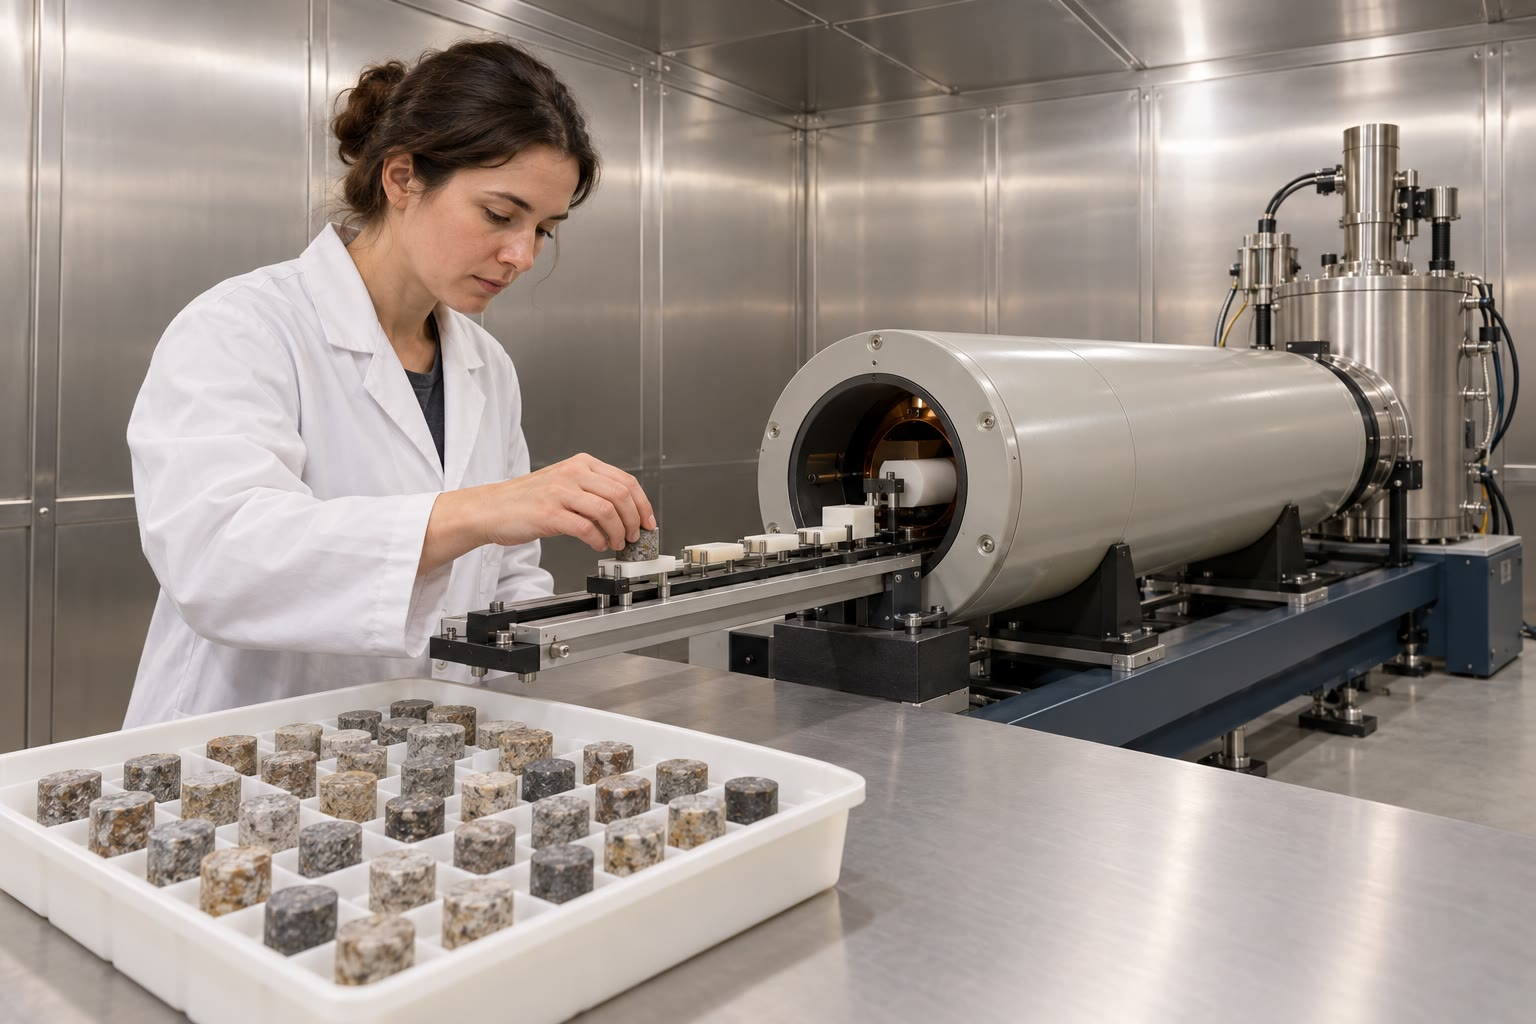
\includegraphics[width=\linewidth]{images/book5/ai/b3-palaeomag-lab.jpg}

{\scriptsize Disposition des échantillons sur le plateau d'un magnétomètre dans une
pièce blindée (illustration générée par IA).}
\end{minipage}
\end{inthelab}

\section{Exercices}

\begin{exercise}[$\star$]\label{exo:b3:palaeomagnetism:1}
Dans un champ de \omterm{def:b3:palaeomagnetism:main-field}{dipôle axial géocentré}, calculer l'inclinaison à la latitude
\ang{30}\,N, et la latitude d'un site où l'inclinaison vaut \ang{-20}.
\end{exercise}

\begin{exercise}[$\star$]\label{exo:b3:palaeomagnetism:2}
À une station, le champ a pour composantes $X = \qty{20000}{nT}$, $Y =
\qty{-2000}{nT}$ et $Z = \qty{40000}{nT}$. Calculer $H$, $F$, la déclinaison
magnétique et l'inclinaison.
\end{exercise}

\begin{exercise}[$\star$]\label{exo:b3:palaeomagnetism:3}
En 2025, $g_1^0 = \qty{-29350}{nT}$. En assimilant le champ à un dipôle axial,
calculer le champ à l'équateur et aux pôles, ainsi que le moment dipolaire
($a = \qty{6371.2}{km}$, $\mu_0 = 4\pi\times\qty{e-7}{H.m^{-1}}$).
\end{exercise}

\begin{exercise}[$\star$]\label{exo:b3:palaeomagnetism:4}
Donner le type d'aimantation rémanente acquise et le moment où elle enregistre le champ, pour~: (a) une
coulée de lave en cours de refroidissement~; (b) des limons se déposant dans un lac calme~; (c) un grès
dont les enduits d'oxydes de fer se transforment en hématite lors d'un enfouissement précoce~;
(d) un basalte resté un million d'années dans le champ actuel.
\end{exercise}

\begin{exercise}[$\star\star$]\label{exo:b3:palaeomagnetism:5}
Quatre échantillons d'un même site donnent les directions $(D, I)$~: $(\ang{12}, \ang{48})$,
$(\ang{22}, \ang{44})$, $(\ang{16}, \ang{57})$ et $(\ang{6}, \ang{53})$.
Calculer leurs vecteurs unitaires, la longueur de la résultante $R$, la direction moyenne, $k$
et $\alpha_{95}$.
\end{exercise}

\begin{exercise}[$\star\star$]\label{exo:b3:palaeomagnetism:6}
Un site à \ang{40.0}\,N, \ang{10.0}\,E donne la direction moyenne $D = \ang{20}$,
$I = \ang{50}$. Calculer sa \omterm{def:b3:palaeomagnetism:vgp}{paléolatitude} et son \omterm{def:b3:palaeomagnetism:vgp}{pôle géomagnétique virtuel}.
\end{exercise}

\begin{exercise}[$\star\star$]\label{exo:b3:palaeomagnetism:7}
Le \omterm{def:b3:palaeomagnetism:igrf}{champ géomagnétique international de référence} (IGRF) donne un moment dipolaire de \qty{8.32e22}{A.m^2} en 1900 et
\qty{7.69e22}{A.m^2} en 2025, et un taux de variation de $g_1^0$ de
\qty{+12.6}{nT/an} en 2025. (a) Calculer la variation relative du moment par
siècle. (b) Si $g_1^0$ conservait ce taux, en combien d'années atteindrait-il zéro~?
Pourquoi ce n'est pas une prévision~?
\end{exercise}

\begin{exercise}[$\star\star$]\label{exo:b3:palaeomagnetism:8}
L'aimantation rémanente restante d'un échantillon, en \unit{mA/m} (nord, est, bas), vaut
$(32.2, 18.1, 38.2)$ après chauffage à \qty{20}{\celsius}, $(25.8, 18.1, 24.6)$
après \qty{300}{\celsius}, et $(0.0, 0.0, 0.0)$ après \qty{580}{\celsius}~; le
\omterm{def:b3:palaeomagnetism:zijderveld}{diagramme de Zijderveld} est rectiligne entre chaque paire. Calculer la direction et
l'intensité de la composante éliminée entre 20 et \qty{300}{\celsius} et de
celle éliminée au-dessus de \qty{300}{\celsius}. Laquelle est la ChRM, et quelle est
l'autre~?
\end{exercise}

\begin{exercise}[$\star\star$]\label{exo:b3:palaeomagnetism:9}
Une formation donne $I = \ang{-35}$ avec $\alpha_{95} = \ang{5}$. Calculer sa
\omterm{def:b3:palaeomagnetism:vgp}{paléolatitude}, l'intervalle de \omterm{def:b3:palaeomagnetism:vgp}{paléolatitudes} compatible avec $I \pm \alpha_{95}$,
et les demi-axes $\mathrm dp$ et $\mathrm dm$ de l'ellipse de confiance de son
pôle.
\end{exercise}

\begin{exercise}[$\star\star\star$]\label{exo:b3:palaeomagnetism:10}
(a) D'après le \cref{thm:b3:palaeomagnetism:dipole}, trouver la latitude à laquelle
l'inclinaison vaut \ang{45}, ainsi que le rapport entre le champ aux pôles et celui
à l'équateur. (b) Montrer que $\mathrm dI/\mathrm d\lambda = 2/(1 + 3\sin^2\lambda)$,
et en déduire où une erreur d'inclinaison donne la plus grande erreur de
\omterm{def:b3:palaeomagnetism:vgp}{paléolatitude}. (c) Pourquoi les \omterm{def:b3:palaeomagnetism:vgp}{paléolatitudes} issues de faibles inclinaisons sont-elles les plus
précises en degrés~?
\end{exercise}

\begin{exercise}[$\star\star\star$]\label{exo:b3:palaeomagnetism:11}
Un site se situe à \ang{35.0}\,S, \ang{150.0}\,E, sur une plaque stable dont le pôle de
référence, pour l'âge d'une formation échantillonnée en ce lieu, se trouve à \ang{70.0}\,N,
\ang{300.0}\,E. (a) Calculer la distance angulaire $p$ entre le site et le pôle,
l'inclinaison et la déclinaison attendues, et la \omterm{def:b3:palaeomagnetism:vgp}{paléolatitude} attendue.
(b) La formation donne $D_o = \ang{30.0}$, $I_o = \ang{-60.0}$. Calculer la
rotation $R$ et le déplacement vers le pôle $P$, et dire ce qu'ils signifient.
\end{exercise}

\begin{exercise}[$\star\star\star$]\label{exo:b3:palaeomagnetism:12}
(a) D'après la \cref{prop:b3:palaeomagnetism:fisher}, montrer que la probabilité
qu'une direction se trouve à moins de $\theta$ de la moyenne soit $(e^\kappa -
e^{\kappa\cos\theta})/(e^\kappa - e^{-\kappa})$. (b) Pour $\kappa$ grand et
$\theta$ petit, montrer que cela vaut environ $1 - e^{-\kappa\theta^2/2}$, et en déduire
que \qty{63}{\percent} des directions se trouvent dans $\theta_{63} \approx
\ang{81}/\sqrt\kappa$. (c) Calculer $\theta_{63}$ pour $\kappa = 50$, et vérifier le
\qty{63}{\percent} avec la formule exacte.
\end{exercise}

\section{Problème~: les couches rouges de Kesta}

\begin{problem}[{Problème du week-end --- trois formations d'un terrane déplacé,
leurs directions, pôles et rotations, et l'âge de la plus jeune}]
\label{pb:b3:palaeomagnetism:1}
% values: calc/ch04.py; palaeomag_stats.py, magnetostratigraphy.py; GPTS: iodp:gpts2004
Kesta est un terrane fictif, aujourd'hui situé à \ang{47.0}\,N, \ang{15.0}\,E, au bord
d'un continent stable fictif. Il affleure trois formations de couches rouges~: A,
\qty{60}{Ma}~; B, \qty{30}{Ma}~; C, d'environ 3.7 à \qty{2.4}{Ma}. Chacune a été
échantillonnée en plusieurs sites, et chaque spécimen a été désaimanté thermiquement~; l'\omterm{def:b3:palaeomagnetism:zijderveld}{aimantation
rémanente caractéristique} (ChRM) est portée par l'hématite, et les formations sont horizontales.

\medskip\noindent\textbf{Partie I --- Directions moyennes.} Les six sites de
la formation A donnent $(D, I)$~: $(\ang{50}, \ang{37})$, $(\ang{28}, \ang{37})$,
$(\ang{21}, \ang{42})$, $(\ang{24}, \ang{27})$, $(\ang{37}, \ang{39})$,
$(\ang{46}, \ang{38})$.
\begin{enumerate}
  \item Pourquoi une ChRM portée par l'hématite dans une couche rouge peut-elle être plus jeune que la
        couche~? Qu'est-ce qui montrerait qu'elle n'est pas beaucoup plus jeune~?
  \item Calculer le vecteur unitaire de la première direction.
  \item Les six vecteurs unitaires ont pour somme $(3.8943, 2.6500, 3.5717)$. Calculer $R$ et
        la direction moyenne de la formation A.
  \item Calculer $k$ et $\alpha_{95}$ pour la formation A.
  \item La formation B donne, à partir de 7 sites, $D = \ang{23.9}$, $I = \ang{51.5}$ et
        $R = 6.8979$~; la formation C, à partir de 8 sites, $D = \ang{3.4}$, $I =
        \ang{63.7}$ et $R = 7.8707$. Calculer $k$ et $\alpha_{95}$ de chacune.
  \item Quelle formation est la mieux groupée~? Quelle moyenne est la mieux définie~?
\end{enumerate}

\medskip\noindent\textbf{Partie II --- Paléolatitudes et pôles.}
\begin{enumerate}[resume]
  \item Calculer les \omterm{def:b3:palaeomagnetism:vgp}{paléolatitudes} de A, B et C.
  \item Pour la formation A, calculer la paléocolatitude $p$ et la latitude de
        son \omterm{def:b3:palaeomagnetism:vgp}{pôle géomagnétique virtuel}.
  \item Calculer la longitude de ce pôle, en vérifiant quel cas du
        \cref{thm:b3:palaeomagnetism:pole} s'applique.
  \item Calculer $\mathrm dp$ et $\mathrm dm$ pour le pôle de A.
  \item Les pôles de B et C se situent à \ang{66.5}\,N, \ang{135.6}\,E et
        \ang{87.1}\,N, \ang{139.1}\,E. Décrire la courbe des trois pôles
        en fonction de l'âge.
\end{enumerate}

\medskip\noindent\textbf{Partie III --- L'âge de la formation C.} Dans la formation C,
à partir de sa base, les spécimens sont inversés jusqu'à \qty{4.2}{m}, normaux jusqu'à
\qty{14.8}{m}, inversés jusqu'à \qty{19.7}{m}, normaux jusqu'à \qty{24.6}{m}, inversés jusqu'à
\qty{29.2}{m} et normaux jusqu'à \qty{54.0}{m}, puis inversés jusqu'au sommet à
\qty{64.0}{m}. Un niveau de cendres à \qty{22}{m} est daté d'environ \qty{3.2}{Ma}. Les
sous-chrons normaux du chron C2An s'étendent de 3.596 à 3.330, de 3.207 à 3.116 et
de 3.032 à \qty{2.581}{Ma}.
\begin{enumerate}[resume]
  \item Faire correspondre les zones de polarité à l'échelle des temps, en utilisant le niveau de cendres.
  \item Calculer le taux d'accumulation entre la première et la troisième
        limite d'inversion, puis entre la quatrième et la sixième.
  \item Estimer les âges de la base et du sommet de la coupe.
  \item Pourquoi le taux est-il une moyenne sur des centaines de milliers d'années, et qu'est-ce qui
        pourrait le faire varier~?
\end{enumerate}

\medskip\noindent\textbf{Partie IV --- Contre le continent stable, et la dérive.} Les
pôles de référence du continent stable se situent à \ang{78.0}\,N, \ang{190.0}\,E
($A_{95} = \ang{3.0}$) à \qty{60}{Ma}~; \ang{83.5}\,N, \ang{175.0}\,E
($\ang{2.5}$) à \qty{30}{Ma}~; et \ang{87.5}\,N, \ang{150.0}\,E ($\ang{2.0}$)
à \qty{4}{Ma}.
\begin{enumerate}[resume]
  \item Calculer la distance angulaire entre Kesta et le pôle de référence
        à \qty{60}{Ma}, ainsi que l'inclinaison et la \omterm{def:b3:palaeomagnetism:vgp}{paléolatitude} attendues.
  \item Calculer la déclinaison attendue à \qty{60}{Ma}.
  \item Les directions attendues à 30 et \qty{4}{Ma} sont $(\ang{2.9},
        \ang{60.0})$ et $(\ang{2.5}, \ang{63.6})$. Calculer le déplacement vers le
        pôle $P$ de A, B et C.
  \item Calculer la rotation $R$ de A, B et C.
  \item Calculer les erreurs $\Delta D_o$ et $\Delta D_x$ pour A, ainsi que l'erreur
        de sa rotation.
  \item Les erreurs de $R$ pour B et C valent \ang{13.8} et \ang{17.9}. Quelles
        rotations sont significatives à \qty{95}{\percent}~?
  \item Raconter l'histoire de Kesta par rapport au continent stable.
  \item Calculer la dérive vers le nord de Kesta depuis la formation A, par rapport à
        l'axe de rotation, en degrés et en kilomètres
        (\qty{111.19}{km} par degré).
  \item Calculer les \omterm{def:b3:palaeomagnetism:vgp}{paléolatitudes} compatibles avec $I \pm \alpha_{95}$ pour
        la formation A, et prendre comme écart-type la moitié de la largeur de
        cet intervalle divisée par 1.96. Donner la dérive vers le nord de Kesta depuis
        A, en kilomètres, avec son écart-type.
\end{enumerate}
\end{problem}
